\interlude[0]{Safety \& Security \\ \Large \hrule \vspace{1.2em} Kulturelle Aspekte}
\section{Safety \& Security}


\SetNextBackground{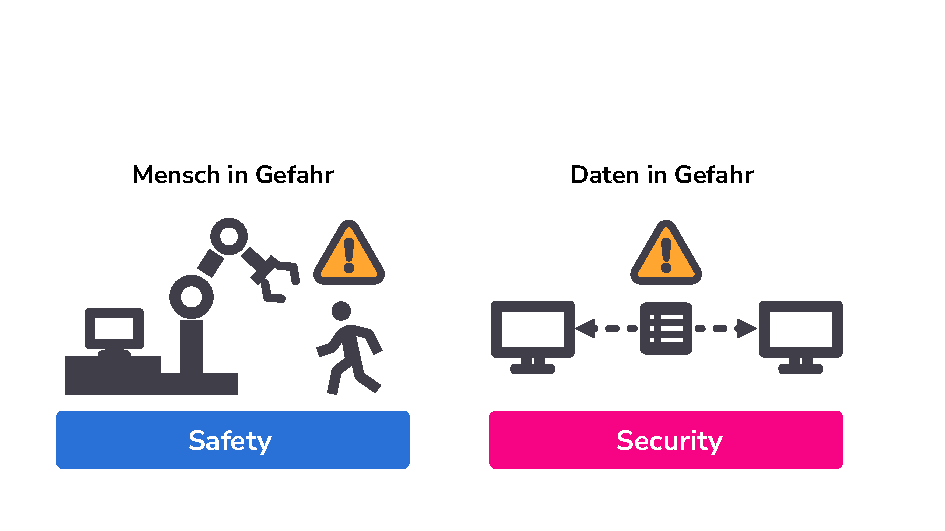
\includegraphics[width=\paperwidth,page=1]{hpke-slide-designs}}
\begin{frame}[T]{Safety \& Security in Computersystemen}
% GOAL Beide Begriffe einführen
%\small
%  \begin{columns}[t,fullwidth]
%   \hfill
%    \begin{column}{.45\linewidth}
%      \begin{block}{Safety}
%      \begin{itemize}
%        \item Schutz von Lebewesen
%      \end{itemize}
%      \end{block}
%    \end{column}
%    \hfill
%    \begin{column}{.45\linewidth}
%      \begin{block}{Security}
%      \begin{itemize}
%        \item Schutz von Informationen
%        \begin{itemize}
%          \item Information vor Dritten geheimhalten
%          \item Information vor Manipulation durch Dritte schützen
%        \end{itemize}
%      \end{itemize}
%      \end{block}
%    \end{column}
%    \hfill
%  \end{columns}
\end{frame}

\begin{frame}[T]{Problemstellungen \& Rahmenbedingungen}
% GOAL Verfahren sind beim ersten Hinblick inkompatibel, Klar machen, dass beide Begriff verschieden sind und verschiedene Vorgehen erfordern
\small

	\begin{tabular}{lllll}
                               & \textbf{Safety}              & \textbf{Security}              \\[1.4em]

  \arrayrulecolor{lightgray}
  \textbf{Fehlerauftreten}     & Zufällig                     & Gezielt (durch Angreifer)      \\[0.35em]
  \midrule                                                                                     \\[-0.75em]
	\textbf{Fehlerbehandlung}    & Weiterbetrieb notwendig      & System stoppen                 \\[0.35em]
  \midrule                                                                                     \\[-0.75em]
  \textbf{Zieldefinition}      & Stabil (Physik bleibt gleich) & In Bewegung (Angreifer lernen)  \\[0.35em]
  \midrule                                                                                     \\[-0.75em]
	\textbf{Abgehangene Sofware} & Stabil!                      & Unsicher?                      \\[0.35em]
  \midrule                                                                                     \\[-0.75em]
	\textbf{Validierungsprozess} & Normiert                     & Dynamisch                      \\
	                             &                              &
	\end{tabular}

  % OLD slide with two-column bullet points
  % \begin{columns}[t,fullwidth]
  %  \hfill
  %   \begin{column}{.45\linewidth}
  %     \begin{block}{Safety}
  %     \begin{itemize}
  %       \item Fehler: Zufällig
  %       \item Im Fehlerfall: Weiterbetrieb ermöglichen!
  %       \item Stabile Zieldefinition:\\Physik bleibt gleich
  %       \item Abgehangene Software $\rightarrow$ Stabil!
  %       \item Normierte Validierungsprozesse
  %     \end{itemize}
  %     \end{block}
  %   \end{column}
  %   \hfill
  %   \begin{column}{.45\linewidth}
  %     \begin{block}{Security}
  %     \begin{itemize}
  %       \item Fehler: Gezielt durch Angreifer
  %       \item Im Fehlerfall: Lieber das System stoppen
  %       \item Zieldefinition ist in Bewegung:\\Angreifer lernen dazu
  %       \item Abgehangene Software $\rightarrow$ Unsicher?
  %       \item Dynamische Validierungsprozesse
  %     \end{itemize}
  %     \end{block}
  %   \end{column}
  %   \hfill
  % \end{columns}
\end{frame}


\begingroup
\ExplSyntaxOn
\definecolor{green1}{RGB}{48, 175, 155}
\definecolor{green2}{RGB}{130, 221, 207}
\colorlet{green3}{rosenpass-lightblue}
\newcommand*{\Level}[1]{
	\str_case:nnF {#1} {
		{+}{
      \begin{tikzpicture}
        \draw[green2] (0,0) circle [radius=0.21];
      \end{tikzpicture}%
		}
		{++}{
      \begin{tikzpicture}[fill=green2,draw=green2]
        \fill (-135\c_colon_str .21) arc [radius=0.21,start~angle=-135,end~angle=45];
        \draw (0,0) circle [radius=0.21];
      \end{tikzpicture}%
    }
		{+++}{
      \begin{tikzpicture}
        \fill[green1] (0,0) circle [radius=0.21];
      \end{tikzpicture}%
    }
    {-}{\raisebox{.08cm}{\color{lightgray!70}\rule[.3\ht\strutbox]{.41cm}{1pt}}}
	}
	{#1}
}
\ExplSyntaxOff

\begin{frame}[T]{Vertrauen schaffen: Akzeptanzkriterien}
  % GOAL erklären, wie man in Safety/Security Konfidenz erzeugt, einen guten Job gemacht zu haben
%  \begin{table}[]
    \begin{tabular}{lrlrl}
      \multirow{2}{*}{}
                          & \multicolumn{2}{c}{\bfseries Safety} & \multicolumn{2}{c}{\bfseries Security} \\[0.2em]
                          &      Konfidenz     &  Verbreitung    &  Konfidenz          &  Verbreitung     \\[0.9em]

    \arrayrulecolor{lightgray}

    Praktische Tests      & \Level{+++}    & \Level{+++}     & \Level{+}           & \Level{++}           \\[-0.10em]
    \midrule                                                                                              \\[-1.20em]
    Proven-in-use         & \Level{++}     & \Level{+}       & \Level{-}           & \Level{+}            \\[-0.10em]
    \midrule                                                                                              \\[-1.20em]
    Mathematische Beweise & \Level{+++}    & \Level{-}       & \Level{+++}         & \Level{++}           \\[-0.10em]
    \midrule                                                                                              \\[-1.20em]
    Externe Audits        & \Level{++}     & \Level{+++}     & \Level{+++}         & \Level{+++}          \\[-0.10em]
    \end{tabular}
    \\[1em]
    \textbf{Verbreitung} Häufigkeit als tragendes Argument im Assurance-Case\\
    \textbf{Konfidenz} Vertrauen in das Kriterium


  % \begin{itemize}
  %   \item Safety
  %   \begin{itemize}
  %     \item Goldstandard: Requirements-getriebenes Testen % üblich
  %     \item Alternative: "Proven in use" % unüblich
  %     \item Alternative: Formale Verifikation % selten
  %   \end{itemize}

  %   \item Security
  %   \begin{itemize}
  %     \item "Proven in use" reicht nicht, aber neuen Verfahren wird dennoch misstraut
  %     \item Testen unzureichend, aufgrund gezielter Angriffe
  %     \item Formale Verifikation ist der Goldweg
  %   \end{itemize}
  % \end{itemize}

\end{frame}
\endgroup

\begin{frame}[T]{Ingenieurskulturen}
  % GOAL Es gibt Unterschiede, die Begründet sind. Wenn Safety und Security verbunden werden sollen, müssen beide Gründe verstanden werden.
	\begin{columns}[t,fullwidth]
		\hfill
		\begin{column}{.45\linewidth}
			\begin{block}{Safety $\Longrightarrow$ Konservativ}
				\begin{itemize}
				\item Menschen Sterben bei Versagen
				\item Probleme sind Verstanden und Stabil
				\end{itemize}
			\end{block}
		\end{column}
		\begin{column}{.45\linewidth}
			\begin{block}{Security $\Longrightarrow$ Progressive}
				\begin{itemize}
				\item Versagen erzeugt eher finanziellen Schaden
				\item Problemtypen sind dynamisch und ändern sich dauernd
				\end{itemize}
			\end{block}
		\end{column}
		\hfill
	\end{columns}

	\begin{columns}[t,fullwidth]
			\hfill
	\begin{column}{\textwidth}
		\hfill\begin{block}{Security + Safety $\Longleftrightarrow$ Konservativ $\lightning$ Progressiv}
	    \begin{itemize}
	      \item Menschen sterben bei Versagen
	      \item Probleme sind dynamisch, Zielsetzung in Bewegung
	    \end{itemize}
  	\end{block}
  			\end{column}
  					\hfill
  	\end{columns}
\end{frame}

\begin{frame}[c]
  % GOAL Klar machen, dass beide Domänen nicht unversöhnbar sind

\addfontfeature{Letters=Uppercase}

	\begin{tcolorbox}[sharp corners,title=Safety + Security: Checkliste,left=.2ex,right=.2ex,toptitle=.5ex,bottomtitle=.5ex]
	\begin{tabular}{@{}>{\stepcounter{enumi}\theenumi.\space}p{\linewidth}@{}}
     Hohe Zuverlässigkeit  \dotfill \CheckedBox\\
     Klarheit über Systemziele \dotfill\CheckedBox\\
     Umfassende Validierung\dotfill\CheckedBox\\
	 Unabhängiges Review\dotfill\CheckedBox\\
     Analyse von Softwaresystemen in reeller Hardware\dotfill\CheckedBox\\
     Redundante Systeme\dotfill\CheckedBox\\
     \textbf{Kryptoagilität} \dotfill\UncheckedBox
	\end{tabular}
	\end{tcolorbox}
	
	\end{frame}
